\documentclass[11pt,a4paper]{article}
\usepackage[T1]{fontenc}
\usepackage[left=2cm, right=2cm, top=2cm, bottom=2cm]{geometry}
\usepackage{graphicx}
\usepackage{mathtools}
\usepackage{amssymb}
\usepackage{amsthm}
\usepackage{thmtools}
\usepackage{xcolor}
\usepackage{nameref}
\usepackage[colorlinks=true, linkcolor=blue, citecolor=cyan]{hyperref}
\usepackage{natbib} 
\usepackage{tkz-graph}
\usepackage{placeins}


\newcommand{\grad}{\operatorname{grad}}
\newcommand{\curl}{\operatorname{curl}}
\renewcommand{\div}{\operatorname{div}}
\newcommand{\img}{\operatorname{img}}
\renewcommand{\span}{\operatorname{span}}
\newcommand{\Z}{\mathbb{Z}}
\newcommand{\tile}[1]{\fbox{{#1}}}



\theoremstyle{definition}
\newtheorem{definition}{Definition}


\theoremstyle{remark}
\newtheorem{remark}{Remark}

\title{Some topological insights to the tiling problem on $ \Z^d $}
\author{Ali Fele Paranj}


\theoremstyle{definition}
\newtheorem{theorem}{Theorem}


\begin{document}
	
	\maketitle
	\begin{abstract}
		In this document I will translates some of the problems in tiling self-assembly to the language of analysis and topology, hoping to open the was for using ergodic theory and other interesting analytical tools. 
	\end{abstract}
	
	
	\section{Introduction}
	
	Let's consider the set of all 2D tiles over the final alphabet $\Sigma$. The set of all such possible tilings is 
	$$ \Sigma^{\mathbb{Z}^2}, $$
	which is the same as the set of all functions from $\mathbb{Z}^2$ to $\Sigma$. 
	
	First, observe that since the alphabet is finite, assuming that it has $N$ elements, then one can write $[n] = \{1,2,3,\cdots,n\}$ in place of $\Sigma$. As far as the set structure of $\Sigma$ is considered, it is fine to do so. However, seeing these two spaces as topological spaces, one automatically assumes a discrete topology over the set $\Sigma$, however, in the case of $[n]$ one automatically assumes that 2 is "close" to 1 and 3 and far from $n$. So we might exploit this topological property of the alphabet set in deciding which tilling is plausible and which is not: based on their gluing structure, that a tile of certain type is willing to be close to the tiles of other type. Then one can possibly encode the plausible tiles as functions that are continuous given the topology of their domain $\mathbb{Z}^2$ and their range $\Sigma$. For more about the intuition behind the method see my notes in this \href{https://github.com/alifele/Lecture-Notes/blob/main/Scientific%20Notes/Some%20Intuitions%20on%20Continuous%20Maps/GraphHomologyAndCohomology.pdf}{link}.
	
	
	\section{Simple Setup}
	Define the $ d_1 $ metric on $ \Z^2 $, where
	\[ d_1\left( (n_1,n_2), (m_1,m_2) \right) = |n_1-n_2| + |m_1-m_2|. \]
	This will induce the topology where the smallest open balls are the Moor neighborhoods (see the first chapter of my \href{https://open.library.ubc.ca/soa/cIRcle/collections/ubctheses/24/items/1.0449873}{thesis} for more on this.) Also assume that we have three types of tiles $ \{ \tile{A}, \tile{B}, \tile{C} \}. $ Assuming that every tile can sit with itself (this can be relaxed later by constructing large enough product space), then the notion of ``certain tiles want to it close to certain other tiles'' will induce a partition on the set of tiles (because it is a equivalence relation). Consider the topology whose sub-basis is this partition of the set. The following figure demonstrates this partition.
	
	\begin{figure}[h!]
	\centering
	
	
	\tikzset{every picture/.style={line width=0.75pt}} %set default line width to 0.75pt        
	
	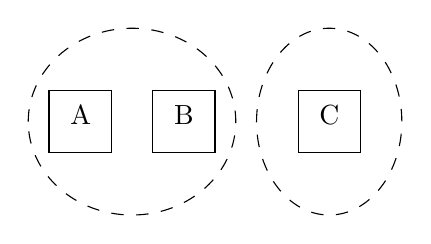
\begin{tikzpicture}[x=0.75pt,y=0.75pt,yscale=-1,xscale=1]
		%uncomment if require: \path (0,300); %set diagram left start at 0, and has height of 300
		
		%Shape: Square [id:dp45846669475066437] 
		\draw   (180,80) -- (210,80) -- (210,110) -- (180,110) -- cycle ;
		%Shape: Square [id:dp8694832240743474] 
		\draw   (230,80) -- (260,80) -- (260,110) -- (230,110) -- cycle ;
		%Shape: Square [id:dp9643149276555201] 
		\draw   (300,80) -- (330,80) -- (330,110) -- (300,110) -- cycle ;
		%Shape: Ellipse [id:dp7472268647554123] 
		\draw  [dash pattern={on 4.5pt off 4.5pt}] (170,95) .. controls (170,70.15) and (192.39,50) .. (220,50) .. controls (247.61,50) and (270,70.15) .. (270,95) .. controls (270,119.85) and (247.61,140) .. (220,140) .. controls (192.39,140) and (170,119.85) .. (170,95) -- cycle ;
		%Shape: Ellipse [id:dp9372300796607134] 
		\draw  [dash pattern={on 4.5pt off 4.5pt}] (280,95) .. controls (280,70.15) and (295.67,50) .. (315,50) .. controls (334.33,50) and (350,70.15) .. (350,95) .. controls (350,119.85) and (334.33,140) .. (315,140) .. controls (295.67,140) and (280,119.85) .. (280,95) -- cycle ;
		
		% Text Node
		\draw (189,86) node [anchor=north west][inner sep=0.75pt]   [align=left] {A};
		% Text Node
		\draw (239,86) node [anchor=north west][inner sep=0.75pt]   [align=left] {B};
		% Text Node
		\draw (309,86) node [anchor=north west][inner sep=0.75pt]   [align=left] {C};
		
		
	\end{tikzpicture}
\end{figure}
	
	Given this ``topology'' on the set of possible tiles, then the following demonstrates two tilings, where the one on the left is a valid tiling, but the one on the right is not a valid tiling.
	
	\begin{figure}[h!]
	\centering
	
	
	\tikzset{every picture/.style={line width=0.75pt}} %set default line width to 0.75pt        
	
	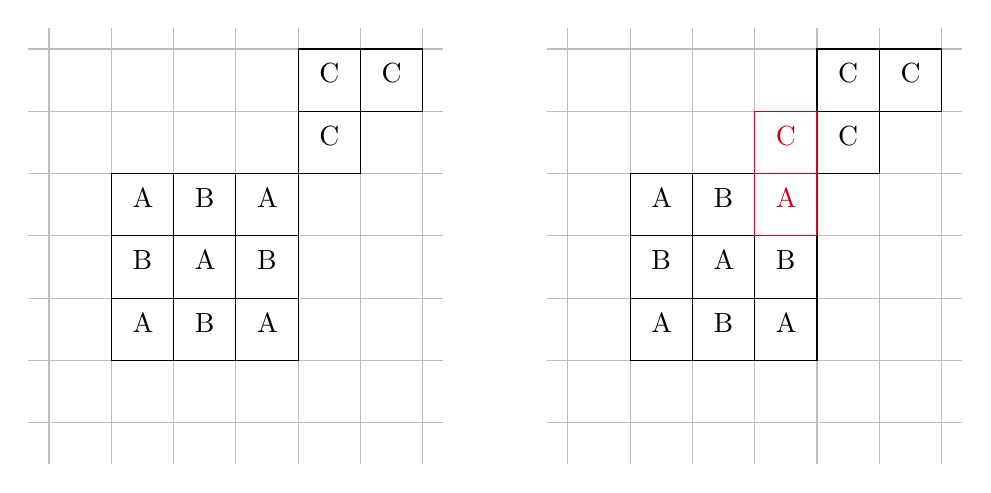
\begin{tikzpicture}[x=0.75pt,y=0.75pt,yscale=-1,xscale=1]
		%uncomment if require: \path (0,300); %set diagram left start at 0, and has height of 300
		
		%Straight Lines [id:da35045523066874695] 
		\draw [color={rgb, 255:red, 190; green, 188; blue, 188 }  ,draw opacity=1 ]   (60,40) -- (60,250) ;
		%Straight Lines [id:da340132848719611] 
		\draw [color={rgb, 255:red, 190; green, 188; blue, 188 }  ,draw opacity=1 ]   (90,40) -- (90,250) ;
		%Straight Lines [id:da9930602253194404] 
		\draw [color={rgb, 255:red, 190; green, 188; blue, 188 }  ,draw opacity=1 ]   (120,40) -- (120,250) ;
		%Straight Lines [id:da673508591738556] 
		\draw [color={rgb, 255:red, 190; green, 188; blue, 188 }  ,draw opacity=1 ]   (150,40) -- (150,250) ;
		%Straight Lines [id:da419114194150617] 
		\draw [color={rgb, 255:red, 190; green, 188; blue, 188 }  ,draw opacity=1 ]   (180,40) -- (180,250) ;
		%Straight Lines [id:da5545224299809445] 
		\draw [color={rgb, 255:red, 190; green, 188; blue, 188 }  ,draw opacity=1 ]   (210,40) -- (210,250) ;
		%Straight Lines [id:da6684800824274905] 
		\draw [color={rgb, 255:red, 190; green, 188; blue, 188 }  ,draw opacity=1 ]   (50,50) -- (250,50) ;
		%Straight Lines [id:da019342059581128557] 
		\draw [color={rgb, 255:red, 190; green, 188; blue, 188 }  ,draw opacity=1 ]   (240,40) -- (240,250) ;
		%Straight Lines [id:da9329975150298714] 
		\draw [color={rgb, 255:red, 190; green, 188; blue, 188 }  ,draw opacity=1 ]   (50,80) -- (250,80) ;
		%Straight Lines [id:da5923754330081309] 
		\draw [color={rgb, 255:red, 190; green, 188; blue, 188 }  ,draw opacity=1 ]   (50,110) -- (250,110) ;
		%Straight Lines [id:da3014815129266917] 
		\draw [color={rgb, 255:red, 190; green, 188; blue, 188 }  ,draw opacity=1 ]   (50,140) -- (250,140) ;
		%Straight Lines [id:da9700279192389916] 
		\draw [color={rgb, 255:red, 190; green, 188; blue, 188 }  ,draw opacity=1 ]   (50,170) -- (250,170) ;
		%Straight Lines [id:da6736918804400827] 
		\draw [color={rgb, 255:red, 190; green, 188; blue, 188 }  ,draw opacity=1 ]   (50,200) -- (250,200) ;
		%Straight Lines [id:da05640786705782641] 
		\draw [color={rgb, 255:red, 190; green, 188; blue, 188 }  ,draw opacity=1 ]   (50,230) -- (250,230) ;
		%Shape: Square [id:dp5803031662244053] 
		\draw   (120,140) -- (150,140) -- (150,170) -- (120,170) -- cycle ;
		
		%Shape: Square [id:dp9196458885257819] 
		\draw   (150,110) -- (180,110) -- (180,140) -- (150,140) -- cycle ;
		
		%Shape: Square [id:dp2648572079254672] 
		\draw   (150,170) -- (180,170) -- (180,200) -- (150,200) -- cycle ;
		
		%Shape: Square [id:dp5425673607779279] 
		\draw   (90,170) -- (120,170) -- (120,200) -- (90,200) -- cycle ;
		
		%Shape: Square [id:dp18348530459906254] 
		\draw   (90,110) -- (120,110) -- (120,140) -- (90,140) -- cycle ;
		
		%Shape: Square [id:dp8856504410510044] 
		\draw   (120,110) -- (150,110) -- (150,140) -- (120,140) -- cycle ;
		
		%Shape: Square [id:dp1873507618967537] 
		\draw   (90,140) -- (120,140) -- (120,170) -- (90,170) -- cycle ;
		
		%Shape: Square [id:dp022117374983126603] 
		\draw   (150,140) -- (180,140) -- (180,170) -- (150,170) -- cycle ;
		
		%Shape: Square [id:dp1634547289103776] 
		\draw   (120,170) -- (150,170) -- (150,200) -- (120,200) -- cycle ;
		
		%Shape: Square [id:dp36442727347773063] 
		\draw   (180,50) -- (210,50) -- (210,80) -- (180,80) -- cycle ;
		%Shape: Square [id:dp5330652912981374] 
		\draw   (210,50) -- (240,50) -- (240,80) -- (210,80) -- cycle ;
		%Shape: Square [id:dp4661865144958631] 
		\draw   (180,80) -- (210,80) -- (210,110) -- (180,110) -- cycle ;
		%Straight Lines [id:da6005649012467171] 
		\draw [color={rgb, 255:red, 190; green, 188; blue, 188 }  ,draw opacity=1 ]   (310,40) -- (310,250) ;
		%Straight Lines [id:da04035283072064799] 
		\draw [color={rgb, 255:red, 190; green, 188; blue, 188 }  ,draw opacity=1 ]   (340,40) -- (340,250) ;
		%Straight Lines [id:da671906501011724] 
		\draw [color={rgb, 255:red, 190; green, 188; blue, 188 }  ,draw opacity=1 ]   (370,40) -- (370,250) ;
		%Straight Lines [id:da49929915066743213] 
		\draw [color={rgb, 255:red, 190; green, 188; blue, 188 }  ,draw opacity=1 ]   (400,40) -- (400,250) ;
		%Straight Lines [id:da6124906908305024] 
		\draw [color={rgb, 255:red, 190; green, 188; blue, 188 }  ,draw opacity=1 ]   (430,40) -- (430,250) ;
		%Straight Lines [id:da17945370773484437] 
		\draw [color={rgb, 255:red, 190; green, 188; blue, 188 }  ,draw opacity=1 ]   (460,40) -- (460,250) ;
		%Straight Lines [id:da6328554243047342] 
		\draw [color={rgb, 255:red, 190; green, 188; blue, 188 }  ,draw opacity=1 ]   (300,50) -- (500,50) ;
		%Straight Lines [id:da6688510350866759] 
		\draw [color={rgb, 255:red, 190; green, 188; blue, 188 }  ,draw opacity=1 ]   (490,40) -- (490,250) ;
		%Straight Lines [id:da612235496519943] 
		\draw [color={rgb, 255:red, 190; green, 188; blue, 188 }  ,draw opacity=1 ]   (300,80) -- (500,80) ;
		%Straight Lines [id:da4514565784776753] 
		\draw [color={rgb, 255:red, 190; green, 188; blue, 188 }  ,draw opacity=1 ]   (300,110) -- (500,110) ;
		%Straight Lines [id:da9360017779771976] 
		\draw [color={rgb, 255:red, 190; green, 188; blue, 188 }  ,draw opacity=1 ]   (300,140) -- (500,140) ;
		%Straight Lines [id:da8873772965675616] 
		\draw [color={rgb, 255:red, 190; green, 188; blue, 188 }  ,draw opacity=1 ]   (300,170) -- (500,170) ;
		%Straight Lines [id:da749590494256885] 
		\draw [color={rgb, 255:red, 190; green, 188; blue, 188 }  ,draw opacity=1 ]   (300,200) -- (500,200) ;
		%Straight Lines [id:da974945622190988] 
		\draw [color={rgb, 255:red, 190; green, 188; blue, 188 }  ,draw opacity=1 ]   (300,230) -- (500,230) ;
		%Shape: Square [id:dp3113813487928936] 
		\draw   (370,140) -- (400,140) -- (400,170) -- (370,170) -- cycle ;
		
		%Shape: Square [id:dp6490479518389014] 
		\draw   (400,170) -- (430,170) -- (430,200) -- (400,200) -- cycle ;
		
		%Shape: Square [id:dp39859172546594845] 
		\draw   (340,170) -- (370,170) -- (370,200) -- (340,200) -- cycle ;
		
		%Shape: Square [id:dp2225864237176991] 
		\draw   (340,110) -- (370,110) -- (370,140) -- (340,140) -- cycle ;
		
		%Shape: Square [id:dp7921412678362084] 
		\draw   (370,110) -- (400,110) -- (400,140) -- (370,140) -- cycle ;
		
		%Shape: Square [id:dp6449792794581529] 
		\draw   (340,140) -- (370,140) -- (370,170) -- (340,170) -- cycle ;
		
		%Shape: Square [id:dp10628620173289283] 
		\draw   (400,140) -- (430,140) -- (430,170) -- (400,170) -- cycle ;
		
		%Shape: Square [id:dp14519260765485775] 
		\draw   (370,170) -- (400,170) -- (400,200) -- (370,200) -- cycle ;
		
		%Shape: Square [id:dp3804583310680284] 
		\draw   (430,50) -- (460,50) -- (460,80) -- (430,80) -- cycle ;
		%Shape: Square [id:dp8462651005127663] 
		\draw   (460,50) -- (490,50) -- (490,80) -- (460,80) -- cycle ;
		%Shape: Square [id:dp23845380767750257] 
		\draw   (430,80) -- (460,80) -- (460,110) -- (430,110) -- cycle ;
		%Shape: Square [id:dp21222113434847067] 
		\draw  [color={rgb, 255:red, 208; green, 2; blue, 27 }  ,draw opacity=1 ] (400,80) -- (430,80) -- (430,110) -- (400,110) -- cycle ;
		%Shape: Square [id:dp188598855194557] 
		\draw  [color={rgb, 255:red, 208; green, 2; blue, 27 }  ,draw opacity=1 ] (400,110) -- (430,110) -- (430,140) -- (400,140) -- cycle ;
		
		
		% Text Node
		\draw (129,146) node [anchor=north west][inner sep=0.75pt]   [align=left] {A};
		% Text Node
		\draw (159,116) node [anchor=north west][inner sep=0.75pt]   [align=left] {A};
		% Text Node
		\draw (159,176) node [anchor=north west][inner sep=0.75pt]   [align=left] {A};
		% Text Node
		\draw (99,176) node [anchor=north west][inner sep=0.75pt]   [align=left] {A};
		% Text Node
		\draw (99,116) node [anchor=north west][inner sep=0.75pt]   [align=left] {A};
		% Text Node
		\draw (129,116) node [anchor=north west][inner sep=0.75pt]   [align=left] {B};
		% Text Node
		\draw (99,146) node [anchor=north west][inner sep=0.75pt]   [align=left] {B};
		% Text Node
		\draw (159,146) node [anchor=north west][inner sep=0.75pt]   [align=left] {B};
		% Text Node
		\draw (129,176) node [anchor=north west][inner sep=0.75pt]   [align=left] {B};
		% Text Node
		\draw (189,56) node [anchor=north west][inner sep=0.75pt]   [align=left] {C};
		% Text Node
		\draw (219,56) node [anchor=north west][inner sep=0.75pt]   [align=left] {C};
		% Text Node
		\draw (189,86) node [anchor=north west][inner sep=0.75pt]   [align=left] {C};
		% Text Node
		\draw (439,56) node [anchor=north west][inner sep=0.75pt]   [align=left] {C};
		% Text Node
		\draw (469,56) node [anchor=north west][inner sep=0.75pt]   [align=left] {C};
		% Text Node
		\draw (439,86) node [anchor=north west][inner sep=0.75pt]   [align=left] {C};
		% Text Node
		\draw (379,176) node [anchor=north west][inner sep=0.75pt]   [align=left] {B};
		% Text Node
		\draw (409,146) node [anchor=north west][inner sep=0.75pt]   [align=left] {B};
		% Text Node
		\draw (349,146) node [anchor=north west][inner sep=0.75pt]   [align=left] {B};
		% Text Node
		\draw (379,116) node [anchor=north west][inner sep=0.75pt]   [align=left] {B};
		% Text Node
		\draw (349,116) node [anchor=north west][inner sep=0.75pt]   [align=left] {A};
		% Text Node
		\draw (349,176) node [anchor=north west][inner sep=0.75pt]   [align=left] {A};
		% Text Node
		\draw (409,176) node [anchor=north west][inner sep=0.75pt]   [align=left] {A};
		% Text Node
		\draw (409,116) node [anchor=north west][inner sep=0.75pt]   [align=left] {\textcolor[rgb]{0.82,0.01,0.11}{A}};
		% Text Node
		\draw (379,146) node [anchor=north west][inner sep=0.75pt]   [align=left] {A};
		% Text Node
		\draw (409,86) node [anchor=north west][inner sep=0.75pt]  [color={rgb, 255:red, 208; green, 2; blue, 27 }  ,opacity=1 ] [align=left] {C};
		
		
	\end{tikzpicture}
\end{figure}
	
	\FloatBarrier
	
	So given the intuition above, one can come up with the following theorem
	
	\begin{theorem}
		In the tiling problem above, a tiling is valid, if and only if its corresponding tiling function is continuous.
	\end{theorem}
	
	
	
	\begin{remark}
		One possible way to formulate this is to assume a discrete topology on $ \Z^2 $, which will force every tiling map to be continuous. However, then, the tiling maps corresponding to valid tiling will precisely be the open maps (the maps that the image of open sets are open sets). 
	\end{remark}
	
	
	\section{Tiles with Glue}
	
	In the example above, we only considered some that some of them want to sit with some other ones and do not sit with certain other ones. However, the way that the tiling problem is formulated in the literature is to assume tiles with different combination of glue values on the sides. I think I can convert this problem to the one similar to above, by considering a sufficiently large product space that captures glue-glue interactions. I know that each glue glue interaction can be captured by a matrix, but I an not certain how to define approporiate topology to convert this formulation to the one similar to above.
	
	
	\subsection{One Possible Formulation}
	
	
	
	
	\section{Discussion}
	One important implication of this approach is that one can easily change the underlying grid structure with hexagonal grids, and etc. 
	
\end{document}